\subsubsection{Introduction}

The aim of this section is to demonstrate the effects of data augmentation on
the performance of the neural network.

\subsubsection{Rational}

Data augmentation is a technique typically used in order to increase the size of
small datasets. Having more images, with unique features allows for the training
of a more robust neural network. By rotating, mirroring, and scaling images the
neural network can become more robust in real use cases to these variances in
input image.

\subsubsection{Design}

For this section, the values in the ``testDataGenerator'' were modified (Figure
\ref{fig:images-Code-dataaug}. The
width shift range and height shift range were given values of 0.1, while the
horizontal and vertical flip arguments were given ``True'' values. The width
shift range and height shift range take a float value and shift the image the
input fraction of the width/height, in this case 1/10th. The horizontal and
vertical flip randomly mirror the image along the horizontal or vertical planes.

No other changes were made to the code from Part a, and a full listing of the
code can be seen in the appendices.

\begin{figure}[H]
	\centering
	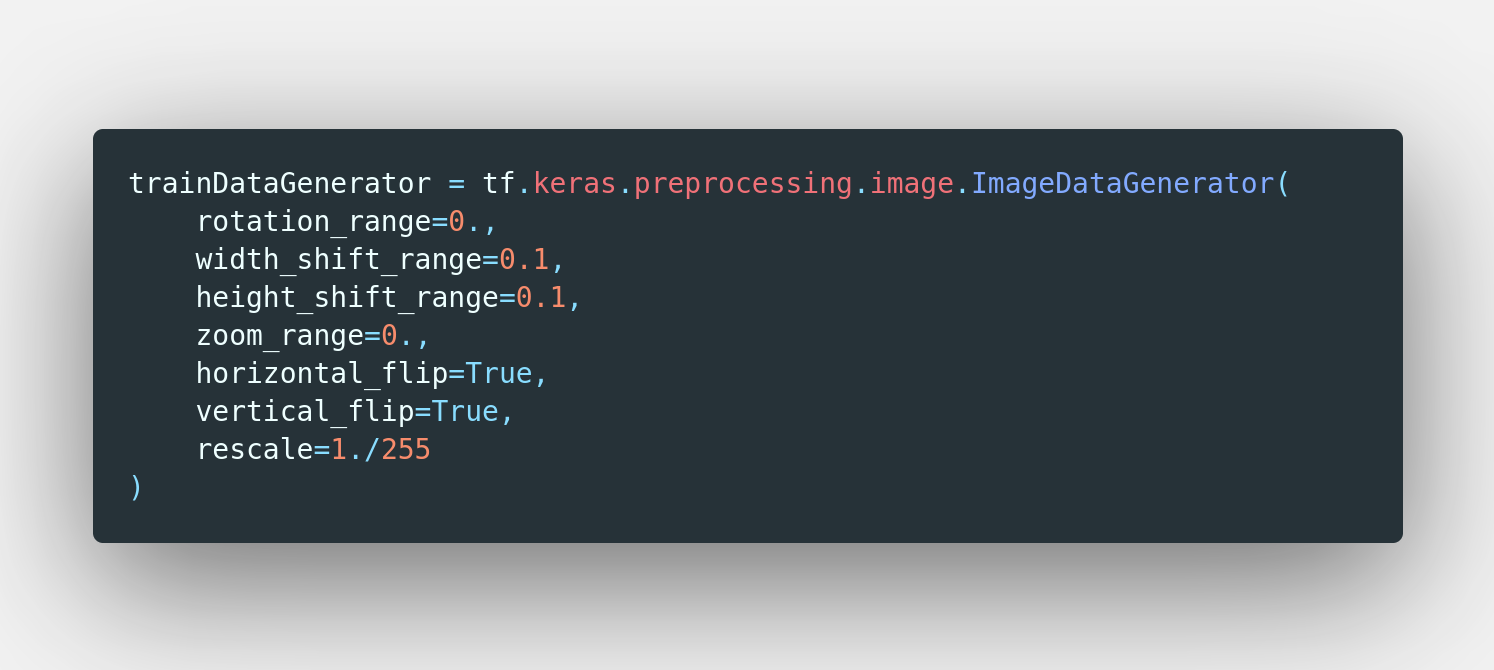
\includegraphics[width=0.8\textwidth]{images/Code/dataaug}
	\caption{Data Augmentation Modifications}
	\label{fig:images-Code-dataaug}
\end{figure}

\subsubsection{Testing}

As there were no hyperparameters being tested, there was no testing which took
place. The code was executed to extract final data, discussed in the Results
section.

\subsubsection{Results}

The output for the neural network structure is the same as that of Part a, as no
change is being made to the CNN structure, only to the input test data.

\begin{figure}[H]
	\centering
	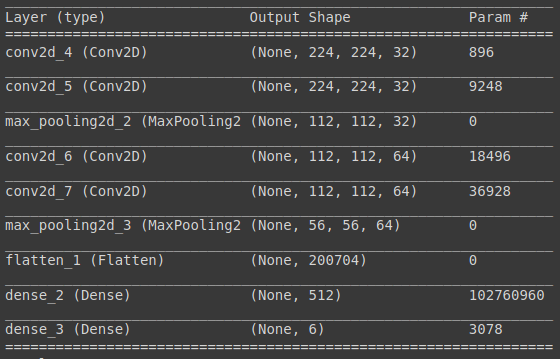
\includegraphics[width=0.8\textwidth]{images/q1/pc/q1pcmodel}
	\caption{Model Summary}
	\label{fig:q1pcmodel}
\end{figure}

Figures \ref{fig:q1pcacc} and \ref{fig:q1pcloss} show that overfitting is not
occurring. While the validation accuracy is quite close to the testing accuracy,
the best fit line through the points on the graph would be below that of the
training accuracy.

\begin{figure}[H]
	\centering
	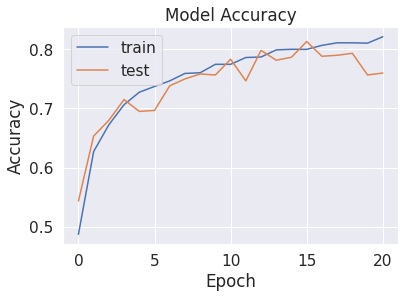
\includegraphics[width=0.8\textwidth]{images/q1/pc/accuracy}
	\caption{Validation and Training Accuracy}
	\label{fig:q1pcacc}
\end{figure}

The loss value improves yet again, with a value of approximately 0.8 in the
validation set.

\begin{figure}[H]
	\centering
	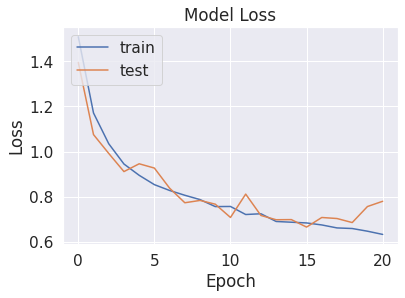
\includegraphics[width=0.8\textwidth]{images/q1/pc/loss}
	\caption{Validation and Training Loss}
	\label{fig:q1pcloss}
\end{figure}

The final output shows an average precision and recall of 85\% and 86\%
respectively , with the highest
values attributed to the ``Parachute'' class, and the lowest values associated
with the ``English Springer'' class.

\begin{figure}[H]
	\centering
	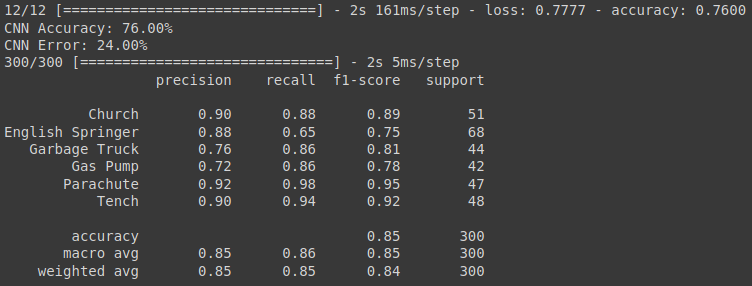
\includegraphics[width=0.8\textwidth]{images/q1/pc/results}
	\caption{Model Testing Results}
	\label{fig:q1pcRes}
\end{figure}

The confusion matrix again demonstrates the number of correctly identified
samples, with the highest precision class being ``Parachute'', labelled as
``4'' within the matrix.

\begin{figure}[H]
	\centering
	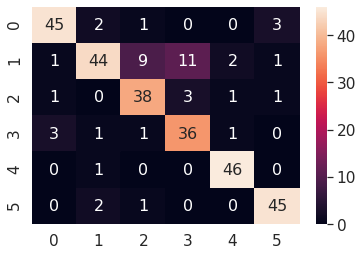
\includegraphics[width=0.8\textwidth]{images/q1/pc/matrix}
	\caption{Confusion Matrix}
	\label{fig:q1pcMatrix}
\end{figure}

Using early stopping, the model ran for a total of 21 epochs. The training time
for this model was 2185.3824 seconds, giving an emission output of 9.106lbs CO2
equivalent emissions. This is, yet again, much higher than Part a, and is also
higher than Part b.
